%% bare_conf.tex
%% V1.3
%% 2007/01/11
%% by Michael Shell
%% See:
%% http://www.michaelshell.org/
%% for current contact information.
%%
%% This is a skeleton file demonstrating the use of IEEEtran.cls
%% (requires IEEEtran.cls version 1.7 or later) with an IEEE conference paper.
%%
%% Support sites:
%% http://www.michaelshell.org/tex/ieeetran/
%% http://www.ctan.org/tex-archive/macros/latex/contrib/IEEEtran/
%% and
%% http://www.ieee.org/

%%*************************************************************************
%% Legal Notice:
%% This code is offered as-is without any warranty either expressed or
%% implied; without even the implied warranty of MERCHANTABILITY or
%% FITNESS FOR A PARTICULAR PURPOSE! 
%% User assumes all risk.
%% In no event shall IEEE or any contributor to this code be liable for
%% any damages or losses, including, but not limited to, incidental,
%% consequential, or any other damages, resulting from the use or misuse
%% of any information contained here.
%%
%% All comments are the opinions of their respective authors and are not
%% necessarily endorsed by the IEEE.
%%
%% This work is distributed under the LaTeX Project Public License (LPPL)
%% ( http://www.latex-project.org/ ) version 1.3, and may be freely used,
%% distributed and modified. A copy of the LPPL, version 1.3, is included
%% in the base LaTeX documentation of all distributions of LaTeX released
%% 2003/12/01 or later.
%% Retain all contribution notices and credits.
%% ** Modified files should be clearly indicated as such, including  **
%% ** renaming them and changing author support contact information. **
%%
%% File list of work: IEEEtran.cls, IEEEtran_HOWTO.pdf, bare_adv.tex,
%%                    bare_conf.tex, bare_jrnl.tex, bare_jrnl_compsoc.tex
%%*************************************************************************

% *** Authors should verify (and, if needed, correct) their LaTeX system  ***
% *** with the testflow diagnostic prior to trusting their LaTeX platform ***
% *** with production work. IEEE's font choices can trigger bugs that do  ***
% *** not appear when using other class files.                            ***
% The testflow support page is at:
% http://www.michaelshell.org/tex/testflow/



\documentclass[conference]{IEEEtran}
% Add the compsoc option for Computer Society conferences.
%
% If IEEEtran.cls has not been installed into the LaTeX system files,
% manually specify the path to it like:
% \documentclass[conference]{../sty/IEEEtran}


% Some very useful LaTeX packages include:
% (uncomment the ones you want to load)

% *** GRAPHICS RELATED PACKAGES ***
%
\usepackage[pdftex]{graphicx}

% *** MATH PACKAGES ***
%
\usepackage[cmex10]{amsmath}

% *** SUBFIGURE PACKAGES ***
%\usepackage[tight,footnotesize]{subfigure}
% subfigure.sty was written by Steven Douglas Cochran. This package makes it
% easy to put subfigures in your figures. e.g., "Figure 1a and 1b". For IEEE
% work, it is a good idea to load it with the tight package option to reduce
% the amount of white space around the subfigures. subfigure.sty is already
% installed on most LaTeX systems. The latest version and documentation can
% be obtained at:
% http://www.ctan.org/tex-archive/obsolete/macros/latex/contrib/subfigure/
% subfigure.sty has been superceeded by subfig.sty.



%\usepackage[caption=false]{caption}
\usepackage[font=footnotesize,caption=false]{subfig}
% subfig.sty, also written by Steven Douglas Cochran, is the modern
% replacement for subfigure.sty. However, subfig.sty requires and
% automatically loads Axel Sommerfeldt's caption.sty which will override
% IEEEtran.cls handling of captions and this will result in nonIEEE style
% figure/table captions. To prevent this problem, be sure and preload
% caption.sty with its "caption=false" package option. This is will preserve
% IEEEtran.cls handing of captions. Version 1.3 (2005/06/28) and later 
% (recommended due to many improvements over 1.2) of subfig.sty supports
% the caption=false option directly:
%\usepackage[caption=false,font=footnotesize]{subfig}
%
% The latest version and documentation can be obtained at:
% http://www.ctan.org/tex-archive/macros/latex/contrib/subfig/
% The latest version and documentation of caption.sty can be obtained at:
% http://www.ctan.org/tex-archive/macros/latex/contrib/caption/


% --------------- USEPACKAGE agregados por guanucoluis ----------------

\usepackage[utf8]{inputenc}
\usepackage{multirow}
%\usepackage[english]{babel}
\usepackage{amssymb}
%\usepackage[pdftex]{graphicx}
\usepackage[hyphenbreaks]{breakurl}
\usepackage[hyphens]{url}
\usepackage{lipsum}


% ------------------------- Agregados por maxi ------------------------

\renewcommand{\abstractname}{Resumen}
\renewcommand{\IEEEkeywordsname}{Palabras claves}
\renewcommand{\figurename}{Fig.}
\renewcommand{\tablename}{Tabla}
\renewcommand{\refname}{Referencias}
\hyphenation{de-sa-rro-llar de-sa-rro-llos}

%lista de posibles "Fixed names"  de latex que pueden hacer falta
%\abstractname	 Abstract
%\alsoname	 see also (makeidx package)
%\appendixname	 Appendix
%\bibname	 Bibliography (report,book)
%\ccname	 cc (letter)
%\chaptername	 Chapter (report,book)
%\contentsname	 Contents
%\enclname	 encl (letter)
%\figurename	 Figure (for captions)
%\headtoname	 To (letter)
%\indexname	 Index
%\listfigurename	 List of Figures
%\listtablename	 List of Tables
%\pagename	 Page (letter)
%\partname	 Partnnn
%\refname	 References (article)
%\seename	 see (makeidx package)
%\tablename	 Table (for caption)



% correct bad hyphenation here
\hyphenation{op-tical net-works semi-conduc-tor}

\begin{document}
%
% paper title
% can use linebreaks \\ within to get better formatting as desired
\title{Servicios REST}


% author names and affiliations
% use a multiple column layout for up to three different
% affiliations
\author{\IEEEauthorblockN{Franco Bocalon, Luis Guanuco, Santiago
    Nolasco}
  \IEEEauthorblockA{Sistemas Distribuidos\\
    Especialidad en Sistemas Embebidos\\
    Instituto Universitario Aeronáutico}
}

% use for special paper notices
%\IEEEspecialpapernotice{(Invited Paper)}


% make the title area
\maketitle


\begin{abstract}
  \lipsum[1]
\end{abstract}

% Note that keywords are not normally used for peerreview papers.
\begin{IEEEkeywords}
Web services, SOAP, REST.
\end{IEEEkeywords}

% IEEEtran.cls defaults to using nonbold math in the Abstract.
% This preserves the distinction between vectors and scalars. However,
% if the conference you are submitting to favors bold math in the abstract,
% then you can use LaTeX's standard command \boldmath at the very start
% of the abstract to achieve this. Many IEEE journals/conferences frown on
% math in the abstract anyway.

% no keywords

% For peer review papers, you can put extra information on the cover
% page as needed:
% \ifCLASSOPTIONpeerreview
% \begin{center} \bfseries EDICS Category: 3-BBND \end{center}
% \fi
%
% For peerreview papers, this IEEEtran command inserts a page break and
% creates the second title. It will be ignored for other modes.
\IEEEpeerreviewmaketitle

\section{Introducción}

Conceptos de SOA. Un diagrama ejemplo con servicios web varios.

Características de SOAP y REST.

\lipsum[7]

\section{SOAP}
\label{sec:soap}

\lipsum[1]

\section{REST}
\label{sec:soap}

%Hablamos del paradigma. Implementación. Un ejemplo
REST o \textsl{Representational State Teansfer} fue creado por Roy
Fielding\footnote{\texttt{http://www.ics.uci.edu/\~fielding/}} en el
año 2000. Este concepto fue expuesto por primera vez en la disertación
de la tesis doctoral de Fielding. En dicha exposición se exploraba
varios estilos arquitectónicos basados en redes. En el Capítulo 5
\cite{FieldingPhD} de sus tesis se hace una descripción profunda. REST
puede ser descrito como una forma de construir servicios Web siguiendo
alguna restricciones entre el proveedor y el cliente de tales
servicios como son\cite{NordicAPIs}:

\begin{itemize}
\item \emph{Mantener separados los intereses entre el cliente y
    servidor}:
  con esto, los clientes no deberían preocuparse por el almacenamiento
  de datos, al igual que los servidores no deben preocuparse por las
  interfaces de usuario. Esto desacopla por completo el desarrollo de
  ambas partes del sistema y permite economizar los recursos en el
  escalamiento. 
\item \emph{La comunicación entre cliente y servidor debería ser ``sin
  estados'' (\emph{stateless})}:  los servidores no deberían almacenar
  ninguna información sobre el contexto del cliente en sus
  llamadas. Obviamente con las excepciones de sesiones que utilizan
  información para mantener la autenticación de la conexión.
\item \emph{Los clientes debe almacenar en cache  las respuestas}:
  todas las
  respuestas del servidor deben conener la suficiente información
  relacionada a cache. Por lo tanto, los clientes puede confiar en esa
  información y decidir por sí mismos qué almacenar de la respuesta en
  cache. 
\item \emph{La conexiones pueden producirse  a través de varias capas de
  comunicación}: los clientes no deben ser capaces de distinguir sí
  están directamente conectados al servidor de la aplicación o a un
  agente intermediario que transmite la información. 
\end{itemize}

\subsection{Simplicidad}
\label{sec:rest-simp}

La simplicidad de REST puede verse en el siguiente ejemplo. Se pide
obtener los datos de un usuario a partir de su identificador. 

Usando la arquitectura SOAP, la petición debería tener la siguiente
forma:

{\footnotesize 
\begin{verbatim}
<?xml version="1.0"?>
<soap:Envelope
xmlns:soap="http://www.w3.org/2001/12/soap-envelope"
soap:encodingStyle="http://www.w3.org/2001/12/soap-encoding">
 <soap:body pb="http://www.acme.com/phonebook">
  <pb:GetUserDetails>
   <pb:UserID>12345</pb:UserID>
  </pb:GetUserDetails>
 </soap:Body>
</soap:Envelope>
\end{verbatim}
}

Esto se envía al servidor utilizando el comando \texttt{HTTP POST}. El
resultado probablemente será probablemente un archivo XML, pero esto
se encuentra embebido como la carga-paga, dentro de una respuesta
SOAP.

Y con REST la consulta probablemente sea como la que sigue,

{\footnotesize 
\begin{verbatim}
http://www.acme.com/phonebook/UserDetails/12345
\end{verbatim}
}

En este caso solo se tiene un URL. Este URL se envía al servidor
usando simplemente un pedido de \texttt{GET} y la respuesta en HTTP se
obtiene en bruto. No se adquiere nada más de lo que se pide al
servidor. 

Note como el método del URL no se llama \texttt{GetUserDetails}, es
simplemente \texttt{UserDetails}. Esto es una de las convenciones en
el diseño REST. Dónde se usa los \emph{sustantivos} en vez de
\emph{verbos}para denotar un simple \emph{recurso}.

\section{Comparación de servicios web}
\label{sec:comparacion}

Aquí vamos a poner las ventajas y desventajas entre los servicios REST
y los web services tradicionales.

\subsection{Casos de uso dónde REST es mejor que SOAP}
\label{sec:cu-rest-better-soap}

SOAP proporciona formas de acceder y manipular objetos de forma
remota, mientras que REST se focaliza en la operaciones que puede ser
ejecutada sobre los recursos. Esta característica hace que REST tenga
mayor adopción en APIs. Además, porque REST hereda operaciones del
protocolo HTTP. Esto último hace fácil la elección de ``cómo abrir una
API web''. Estas características han influido tanto que grandes
compañías Web utilizan la API REST\footnote{RESTful es el nombre
  técnico de la implementación de REST.}.

REST es mejor que SOAP en situaciones que no requieren un mapeo total
de los objetos, al cliente. La comunicación de información de objetos
en ambos sentidos demanda una cantidad importante de ancho de banda,
lo que podría ser una limitante en entornos donde la conectividad es
costosa. Una API requerida principalmente para aplicaciones móviles is
uno de los casos de uso dónde se debe evitar el uso de SOAP a todo
costo. 

Otro factor en la preferencia a REST es la simplicidad de la
implementación con respecto a SOAP. También, al ser menos restrictivo
que SOAP, algunos APIs de REST trabajan mejor en la actualidad. En
algunos casos los desarrolladores no conocen en profundidad los
contratos a la hora de implementar una API. Las APIs públicas cambian
constantemente debido a las necesidades de negocio y son adaptables
rápidamente. En esta situación REST resulta una elección
natural. El uso de SOAP en las condiciones expuestas sería
contraproducente, ya que podría introducir una complejidad contractual
innecesaria. 

\section{Implementación RESTful}
\label{sec:imp-rest}

Presentar un caso sencillo de RESTful (implementación de REST).

\lipsum[3]


\section{Conclusiones}
\label{sec:con}


\begin{table}[!t]
\renewcommand{\arraystretch}{1.3}
\caption{Recursos de hardware en función de los niveles de aprendizaje}
\label{tab:rec-plataforma}
\centering
\begin{tabular}{|l|c|c|c|}
\hline
\multirow{2}{*}{Nivel} & Llaves/pulsadores & ADC\&DAC/SPI & USB/ETH \\
                       & Diodos LED & Display LCD/VGA & HDMI \\
\hline
Inicial & $\checkmark$ & & \\
\hline
Medio & $\checkmark$ & $\checkmark$ & \\
\hline
Avanzado & $\checkmark$ & $\checkmark$ & $\checkmark$ \\
\hline
\end{tabular}
\end{table}

\lipsum[3-4]

\begin{figure}[!t]
  \centering
  \subfloat[BASYS2 (Digilent)]{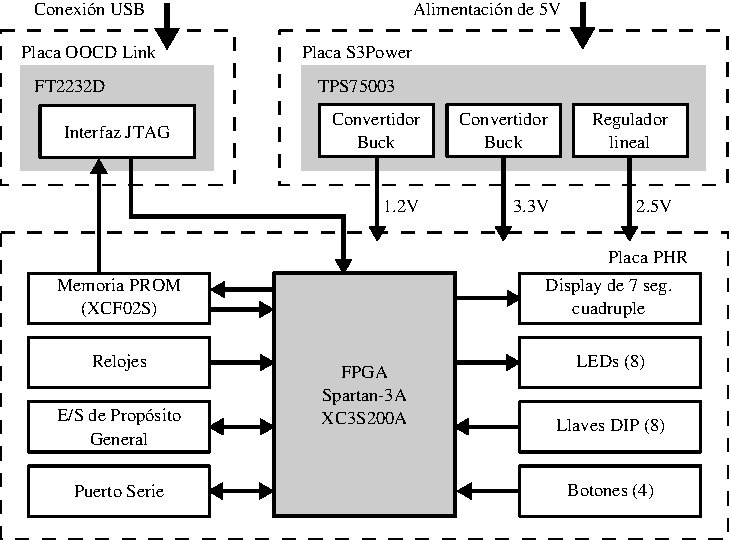
\includegraphics[width=0.2\textwidth]{img/block}%  
    \label{fig:digilent-board}}
  \hfil
  \subfloat[DE0-Nano (Altera)]{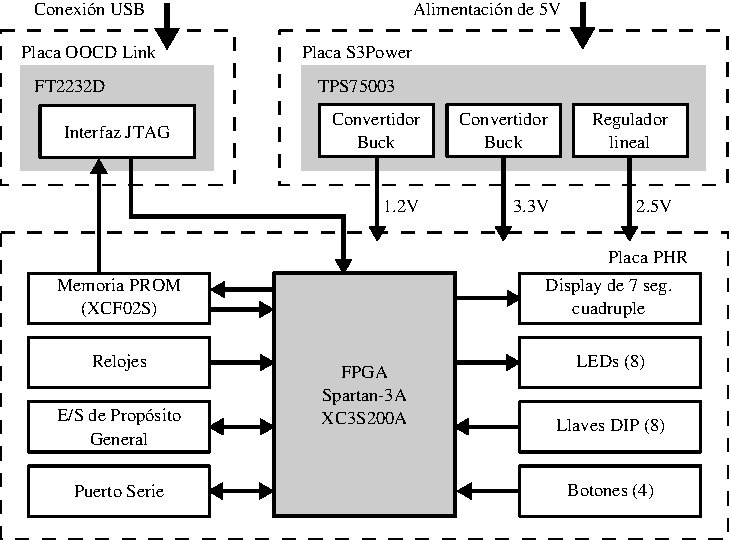
\includegraphics[width=0.2\textwidth]{img/block}%
    \label{fig:altera-board}}
  \hfil
  \subfloat[Avnet Spartan-6 LX150T (Xilinx/Avnet)]{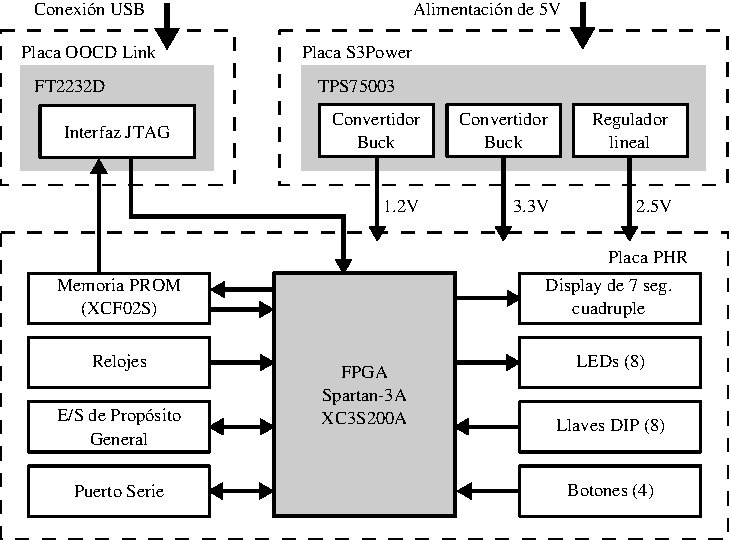
\includegraphics[width=0.2\textwidth]{img/block}%
    \label{fig:xilinx-board}}
  \caption{Plataformas comerciales de desarrollo educativas basadas en FPGAs.}
  \label{fig:board-fpga}
\end{figure}

\lipsum[6]

\begin{table}[!t]
%increase table row spacing, adjust to taste
\renewcommand{\arraystretch}{1.3}
% if using array.sty, it might be a good idea to tweak the value of
% \extrarowheight as needed to properly center the text within the cells
\caption{Característica de la familia Spartan-3A}
\label{tab:char-fpga}
\centering
% Some packages, such as MDW tools, offer better commands for making tables
% than the plain LaTeX2e tabular which is used here.
\begin{tabular}{|l|c|c|c|c|}
\hline
\multirow{2}{*}{\textbf{Devices}} & \textbf{System} & \textbf{Block RAM} & \textbf{Dedicated} &  \textbf{Maximum} \\
 & \textbf{Gates} & \textbf{bits} & \textbf{Multipliers} & \textbf{User I/O} \\
\hline
XC3S50A & 50K & 54K & 3 & 144 \\
\hline
\textbf{XC3S200A} & \textbf{200K} & \textbf{288K} & \textbf{16} & \textbf{248} \\
\hline
XC3S400A & 400K & 360K & 20 & 311 \\
\hline
XC3S700A & 700K & 360K & 20 & 372 \\
\hline
XC3S1400A & 1400K & 576K & 32 & 502 \\
\hline
\end{tabular}
\end{table}

\begin{table}[!t]
\renewcommand{\arraystretch}{1.3}
\caption{Tipo de memoria para la familia Spartan-3A}
\label{tab:mem-fpga}
\centering
\begin{tabular}{|l|c|c|}
\hline
\multirow{2}{*}{\textbf{Devices}} & \textbf{Configuration} & \textbf{ISP PROM} \\
 & \textbf{Bits} & \textbf{Solution} \\
\hline
XC3S50A   & 437,312   & XCF01S \\
\hline                        
\textbf{XC3S200A}  & \textbf{1,196,128} & \textbf{XCF02S} \\
\hline                        
XC3S400A  & 1,886,560 & XCF02S \\
\hline                        
XC3S700A  & 2,732,640 & XCF04S \\
\hline
XC3S1400A & 4,755,296 & XCF08P     \\
\hline
\end{tabular}
\end{table}

\begin{figure}[!t]
\centering
  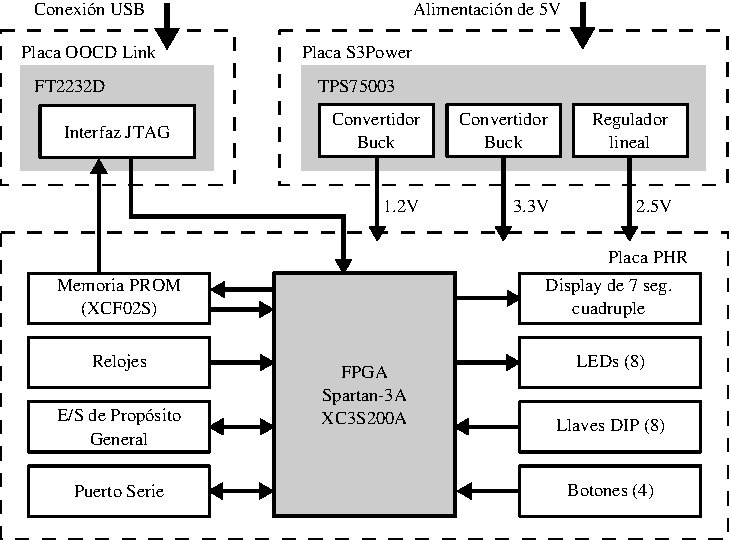
\includegraphics[width=0.45\textwidth]{img/block}
  \caption{Diagrama en bloque de la PHR.}
  \label{fig:phr-bloque}
\end{figure}


\begin{figure}[!t]
  \centering
  \subfloat[Placa PHR (base)]{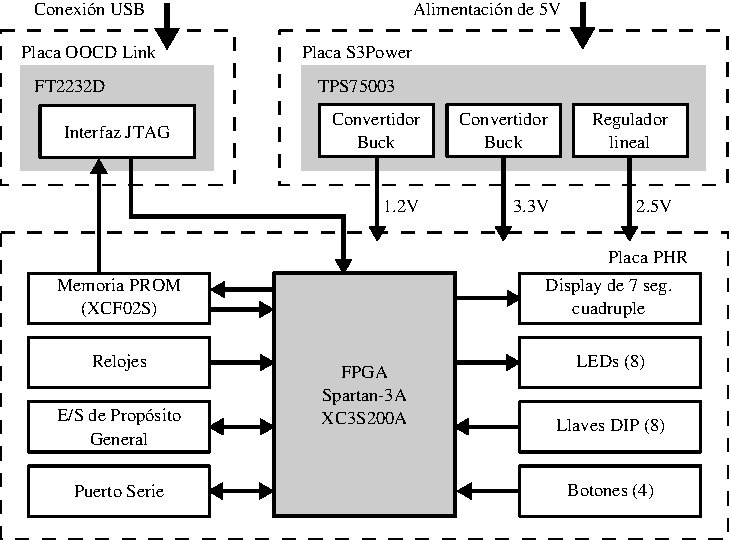
\includegraphics[width=0.4\textwidth]{img/block}%  
    \label{fig:foto-phr}}
  \hfil
  \subfloat[Placa S3Power]{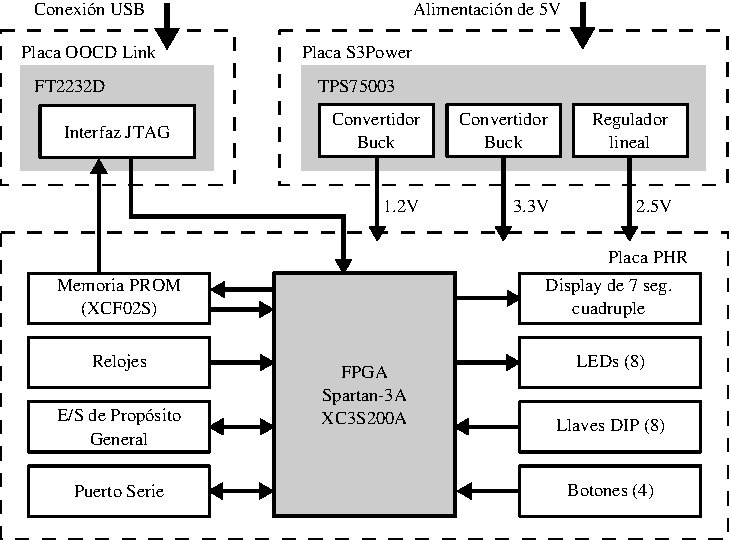
\includegraphics[width=0.2\textwidth]{img/block}%
    \label{fig:foto-s3power}}
  \hfil
  \subfloat[Conexión PHR-S3Power]{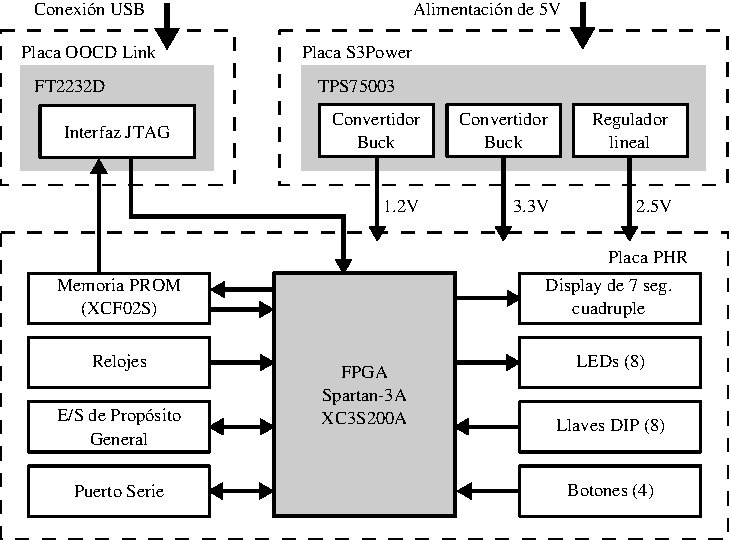
\includegraphics[width=0.25\textwidth]{img/block}%
    \label{fig:foto-phr-s3power}}
  \caption{Placas PHR y S3Power.}
  \label{fig:placas-phr-s3power-con}
\end{figure}

\section{Interfaz JTAG}
\label{sec:jtag}

\lipsum[45-48]

\begin{figure*}[!t]
  \centerline{\subfloat[Esquema de la  FT2232D]{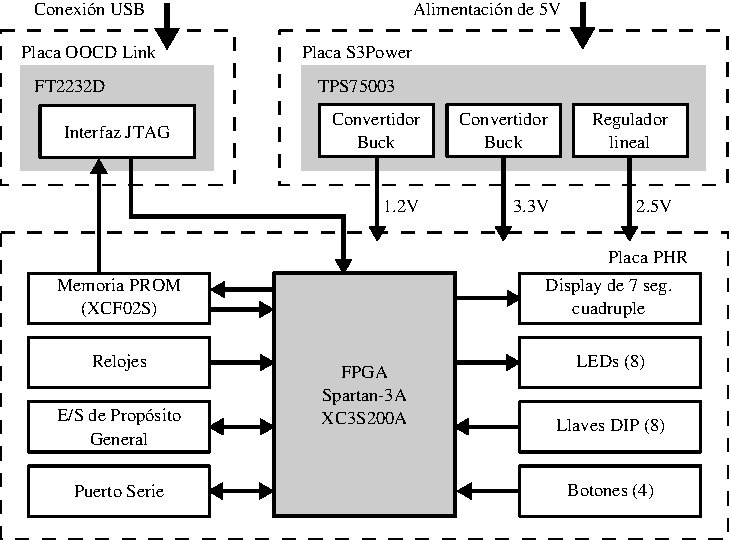
\includegraphics[width=0.35\textwidth]{img/block}%  
    \label{fig:oocdlink-bloque}}
  \hfil
  \subfloat[Placa OOCDLink]{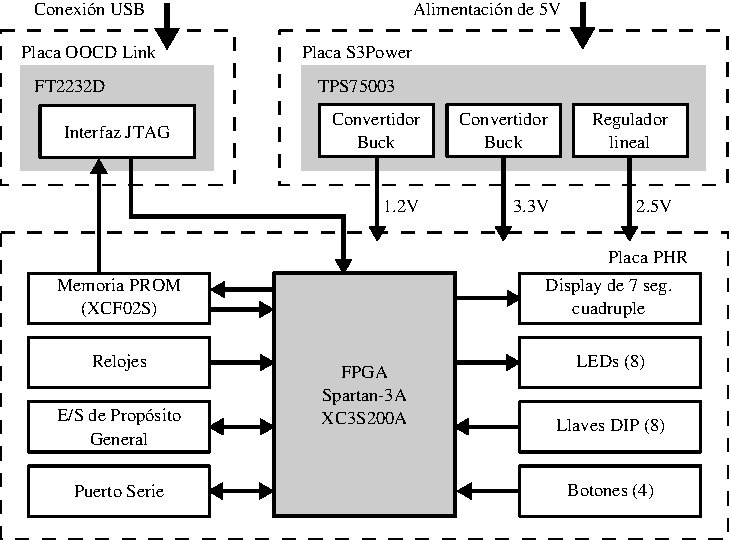
\includegraphics[width=0.2\textwidth]{img/block}%
    \label{fig:oocdlink-foto}}
  \hfil
  \subfloat[Conexión entre la placa PHR y OOCDLink]{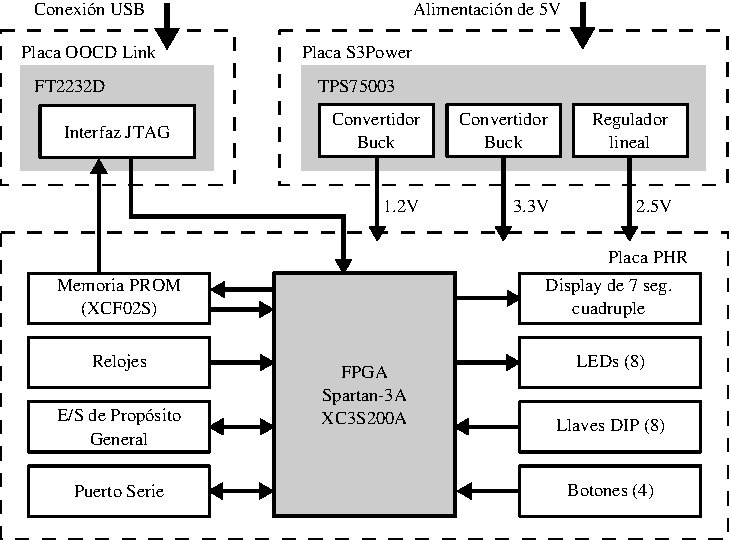
\includegraphics[width=0.4\textwidth]{img/block}%
    \label{fig:oocdlink-phr}}}
  \caption{Interfaz JTAG (implementación FT2232D).}
  \label{fig:oocdlink}
\end{figure*}

\section*{Agradecimientos}

\lipsum[75-80]

\begin{thebibliography}{1}

% \bibitem{IEEEhowto:kopka}
% H.~Kopka and P.~W. Daly, \emph{A Guide to \LaTeX}, 3rd~ed.\hskip 1em plus
%   0.5em minus 0.4em\relax Harlow, England: Addison-Wesley, 1999.

\bibitem{FieldingPhD}
  Roy~Fielding, \emph{Architectural Styles and the Design of
    Network-based Software Architectures}. University of California,
  Irvine. 2000. url:\texttt{\burl{http://www.ics.uci.edu/~fielding/pubs/dissertation/rest_arch_style.htm}}.

\bibitem{NordicAPIs}
Bruno Pedro, \emph{Is REST better than SOAP? Yes, in Some Use Cases},
url:
\texttt{\burl{http://nordicapis.com/rest-better-than-soap-yes-use-cases/}}.

\bibitem{LearnREST}
  Dr. M. Elkstein, \emph{Learn REST: A Tutorial},
url: \texttt{\burl{http://rest.elkstein.org/}}.




\end{thebibliography}

% that's all folks
\end{document}


